% Deze template is gemaakt door Fons van der Plas (f.vanderplas@student.ru.nl) voor het publiek domein en mag gebruikt worden **zonder vermelding van zijn naam**.
% This template was created by Fons van der Plas (f.vanderplas@student.ru.nl) for the public domain, and may be used **without attribution**.
\documentclass{article}
\usepackage[utf8]{inputenc}     % for éô
\usepackage[english]{babel}     % for proper word breaking at line ends
\usepackage[a4paper, left=1.5in, right=1.5in, top=1.5in, bottom=1.5in]{geometry}
                                % for page size and margin settings
\usepackage{graphicx}           % for ?
\usepackage{amsmath,amssymb}    % for better equations
\usepackage{amsthm}             % for better theorem styles
\usepackage{mathtools}          % for greek math symbol formatting
\usepackage{enumitem}           % for control of 'enumerate' numbering
\usepackage{listings}           % for control of 'itemize' spacing
\usepackage{todonotes}          % for clear TODO notes
\usepackage{hyperref}           % page numbers and '\ref's become clickable
\usepackage{etoolbox}
\usepackage{lipsum}   % for filler text
\usepackage{setspace}
\usepackage{caption}
\usepackage{subcaption}
\AtBeginEnvironment{quote}{\singlespacing\small}

%%%%%%%%%%%%%%%%%%%%%%%%%%%%%%%%
%% SET TITLE PAGE VALUES HERE %%
%%%%%%%%%%%%%%%%%%%%%%%%%%%%%%%%
%             ||               %
%             ||               %
%             \/               %

\def\thesistitle{Convolutional Neural Networks applied to Keyword Spotting using Transfer Learning}
\def\thesissubtitle{Why Transfer learning is worth a try}
\def\thesisauthorfirst{Christoph}
\def\thesisauthorsecond{Schmidl}
\def\thesisauthorstudentnumber{s4226887}
\def\thesisauthoremail{c.schmidl@student.ru.nl}
\def\thesissupervisorfirst{dr. L.F.M. }
\def\thesissupervisorsecond{ten Bosch}
\def\thesissecondreaderfirst{prof. dr. Louie}
\def\thesissecondreadersecond{Duck}
\def\thesisdate{\today}


%             /\               %
%             ||               %
%             ||               %
%%%%%%%%%%%%%%%%%%%%%%%%%%%%%%%%
%% SET TITLE PAGE VALUES HERE %%
%%%%%%%%%%%%%%%%%%%%%%%%%%%%%%%%


%% FOR PDF METADATA
\title{\thesistitle}
\author{\thesisauthorfirst\space\thesisauthorsecond}
\date{\thesisdate}

%% TODO PACKAGE
\newcommand{\towrite}[1]{\todo[inline,color=yellow!10]{TO WRITE: #1}}

%% THEOREM STYLES
\newtheorem{theorem}{Theorem}[section]
\newtheorem{corollary}{Corollary}[theorem]
\newtheorem{lemma}[theorem]{Lemma}
\newtheorem{proposition}[theorem]{Proposition}

\theoremstyle{definition}
\newtheorem{definition}[theorem]{Definition}

\theoremstyle{remark}
\newtheorem*{remark}{Remark}



%% MATH OPERATORS
\DeclareMathOperator{\supersine}{supersin}
\DeclareMathOperator{\supercosine}{supercos}

%%%%%%%%%%%%%%%%%%%%%%%

\begin{document}
\begin{titlepage}
	\thispagestyle{empty}
	\newcommand{\HRule}{\rule{\linewidth}{0.5mm}}
	\center
	\textsc{\Large Radboud University Nijmegen}\\[.7cm]
	
\includegraphics[width=25mm]{img/in_dei_nomine_feliciter.eps}\\[.5cm]
	\textsc{Faculty of Science}\\[0.5cm]
	
	\HRule \\[0.4cm]
	{ \huge  \thesistitle}\\[0.1cm]
	%\textsc{\thesissubtitle}\\
	\HRule \\[.5cm]
	

	\textsc{\large Thesis in Automatic Speech Recognition (LET-REMA-LCEX10)}\\[.5cm]

% https://tex.stackexchange.com/questions/81955/align-text-in-minipage-at-same-height
	\begin{minipage}[t]{0.4\textwidth}
	\begin{flushleft} \large
	\emph{Author:}\\
	\vspace{1em}
	\thesisauthorfirst\space \textsc{\thesisauthorsecond}\\
	\thesisauthorstudentnumber\\
	\thesisauthoremail\space 
	\end{flushleft}
	\end{minipage}
	~
	\begin{minipage}[t]{0.4\textwidth}
	\begin{flushright} \large
	\emph{Supervisor:} \\
	\vspace{1em}
	\thesissupervisorfirst\space \textsc{\thesissupervisorsecond} \\[1em]
	%\emph{Second reader:} \\
	%\thesissecondreaderfirst\space \textsc{\thesissecondreadersecond}
	\end{flushright}
	\end{minipage}\\[4cm]
	\vfill
	{\large \thesisdate}\\
	\clearpage
\end{titlepage}

\tableofcontents

\newpage

\section{Introduction}

The task of keyword spotting (KWS) is interesting to different domains where a hands-free interaction experience is required or desired like Google's feature of interacting with mobile devices (include "OK Google" reference). \\

Different approaches to keyword spotting like:

\begin{itemize}
	\item Deep Neural Networks (DNNs)
	\item Convolutional Neural Networks (CNNs)
	\item (Keyword/Filler) Hiddem Markov Models (HMMs)
\end{itemize}



\begin{enumerate}
	\item Problem
	\item Background (literature overview)
	\item Research Question, Hypotheses, intro to experiment
\end{enumerate}

\subsection{Literature review}

This section contains the most prominent approaches to the KWS task which have been successfully applied in the past and serve as baseline models or inspirations for the proposed model in this thesis. 

\subsubsection{Raw waveform-based audio classification using sample-level CNN architectures}

\begin{itemize}
	\item Raw waveform-based audio classification using sample-level CNN architectures \cite{lee2017raw}
\end{itemize}


\subsubsection{Transferable deep features for keyword spotting}


\begin{itemize}
	\item Transferable deep features for keyword spotting \cite{retsinas2018transferable}
\end{itemize}

\subsubsection{Imagenet: A large-scale hierarchical image database}

\begin{itemize}
	\item Imagenet: A large-scale hierarchical image database \cite{deng2009imagenet}
\end{itemize}


\subsubsection{Imagenet classification with deep convolutional neural networks}

\begin{itemize}
	\item Imagenet classification with deep convolutional neural networks \cite{krizhevsky2012imagenet}
\end{itemize}

\subsubsection{Speech Recognition: Keyword Spotting Through Image Recognition.}

The authors of the paper "Speech Recognition: Keyword Spotting Through Image Recognition" \cite{gouda2018speech} transformed the KWS task which incoporates audio data into the domain of image classification. They used the Speech Commands Dataset \cite{warden2018speech} which contains spoken words of the length of one second in order to train and evalutate their model. According to \cite{warden2018speech}, the Speech Commands Dataset V2 \cite{scd_v2} comprises one-second audio clips which were sampled at 16KHz and containing ten words, namely "Yes", "No", "Up", "Down", "Left", "Right", "On", "Off", "Stop", and "Go", and have one additional special label for "Unknown Word", and another for "Silence" (no speech detected). A vector representation of these one-second audio clips would therefore be of the form  $\mathbb{R}^{16000}$.\\

The authors used three different models, namely:

\begin{itemize}
	\item A Low Latency Convolutional Neural Network which is designed to reduce its memory footprint by limiting the number of model parameters. This model is similar to the model called "cnn-one-fstride4" which is used in \cite{sainath2015convolutional} but differs in terms of filter size, stride, channels, dense and params. The model has been trained using Stochastic Gradient Descent and Xavier Initialization has been used in order to initialize the model weights.
	\item The MNIST TensorFlow CNN / Basic CNN where some tweaks have been performed to the first layer in order to fix dimension mismatches. A baseline architecture is described in \cite{sainath2015convolutional} (3 module setup?).
	
		\begin{itemize}
			\item \url{https://github.com/tensorflow/docs/blob/master/site/en/tutorials/estimators/cnn.ipynb}
			\item \url{https://github.com/tensorflow/tensorflow/tree/master/tensorflow/examples/tutorials/mnist}
		\end{itemize}
		
		\item Adversarially trained CNN which is inspired by MCDNN \cite{cirecsan2012multi} and AlexNet \cite{krizhevsky2012imagenet}. One shallow CNN which has been used for prototyping and hyperparameter tuning. Dropout was counter-productive and therefore Virtual Adversarial Training was used, inspired by \cite{goodfellow2016deep}.
		
\end{itemize}

Evaluated parameters in this paper:

\begin{itemize}
	\item Adversarial Training Results and Comparison with
Vanilla CNN
	\item increase in training and validation accuracy over the first ten epochs for the low-latency convolution and VAT models: a zoomed-in version of Figure 12
	\item decrease of costs over 500 epochs for the lowlatency convolution and VAT models: a zoomed-out version of Figure 13
	\item  increase of training and validation accuracy over 500 epochs for the low-latency convolution and VAT models: a zoomed-out version of Figure 10
	\item  reduction of cost over the first ten epochs for the low-latency convolution and VAT models: a zoomed-in version of Figure 11
	\item the evolution of training cross-entropy loss (blue and green) and validation accuracy (red and orange) compared between Xavier and truncated normal initialization; Xavier converges much faster and may attain better results
	\item the evolution of training cross-entropy loss (blue and green) and validation accuracy (red and orange) compared between Adam and SGD optimization; Adam converges faster than SGD but reaches the same results
	\item  effect of the number of frequency-counting buckets on the accuracy of the low-latency convolution model. The model did not benefit from the increase in available data caused by increasing the number of buckets.
	\item effect of the spectrogram window size on the accuracy of the low-latency convolution model. There is a local optimum, as there was for stride in Figure 18.
	\item effect of added background noise on the final accuracy of the low-latency convolution model. The horizontal axis is signal-noise ratio in linear units.
	\item effect of the spectrogram window stride on the accuracy of the low-latency convolution model. For low values of stride, there is too much redundancy, while larger values result in lost information.
\end{itemize}

\textbf{Conlusion}

In this project we tackled the speech recognition problem by applying different CNN models on image data formed using log spectrograms of the audio clips. We also successfully implemented a regularization method "Virtual Adversarial Training" that achieved a maximum of 92\% validation accuracy on 20\% random sample of
the input data.\\
The significant work done in this project was the demonstration of how to convert a problem in audio recognition into the better-studied domain of image classification, where the powerful techniques of convolutional neural networks are fully developed.
We also saw, particularly in the case of the low-latency convolution model, how crucial good hyperparameter tuning is to the accuracy of the model. A great number of hyperparameters must be tuned, including the many choices that go into network architecture, and any of the hyperparameters, poorly chosen, can make or break the overall performance of the model. Another contribution was the use of adversarial training to provide a regularization effect in audio recognition; this technique improved results relative even to well-established techniques such as dropout, and therefore has promising applications in the future.



\begin{figure}
\centering
\begin{subfigure}{.5\textwidth}
  \centering
  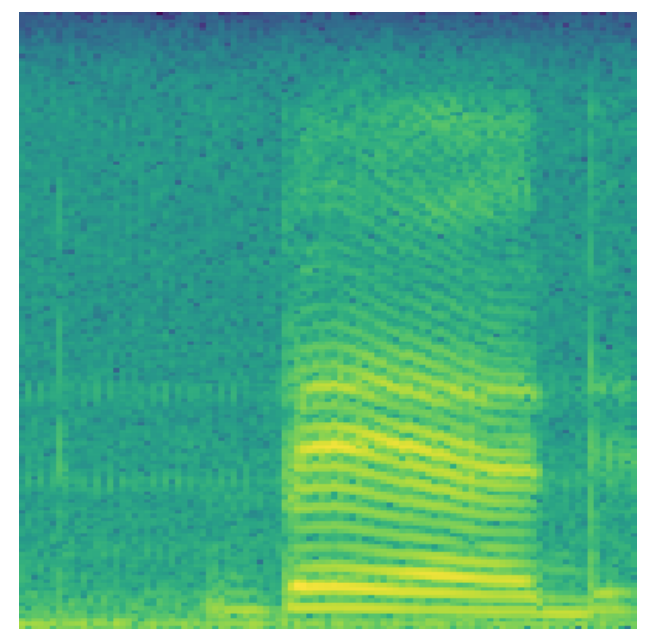
\includegraphics[width=.5\linewidth]{img/papers/image_recognition/spectrogram.png}
  \caption{}
  \label{fig:sub1}
\end{subfigure}%
\begin{subfigure}{.5\textwidth}
  \centering
  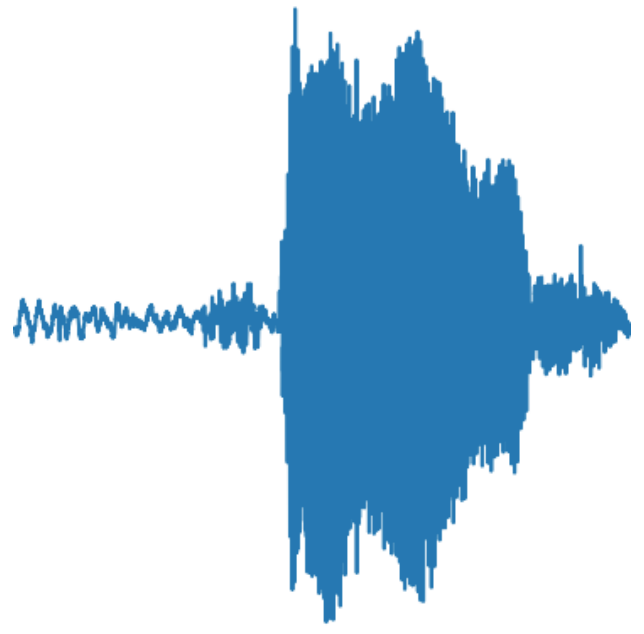
\includegraphics[width=.5\linewidth]{img/papers/image_recognition/amplitude_vs_time.png}
  \caption{}
  \label{fig:sub2}
\end{subfigure}
\caption{A comparison of the spectrogram (a) and the
amplitude-vs.-time plot (b) for the same audio recording of
a person saying the word “bed”.}
\label{fig:test}
\end{figure}



\textcolor{red}{Include summary about the approach of converting the long, one dimensional vector of audio data into a spectrograms and therefore making it a image classification problem.}

\subsubsection{Convolutional neural networks for small-footprint keyword spotting}

\begin{figure}[h]
    \centering
    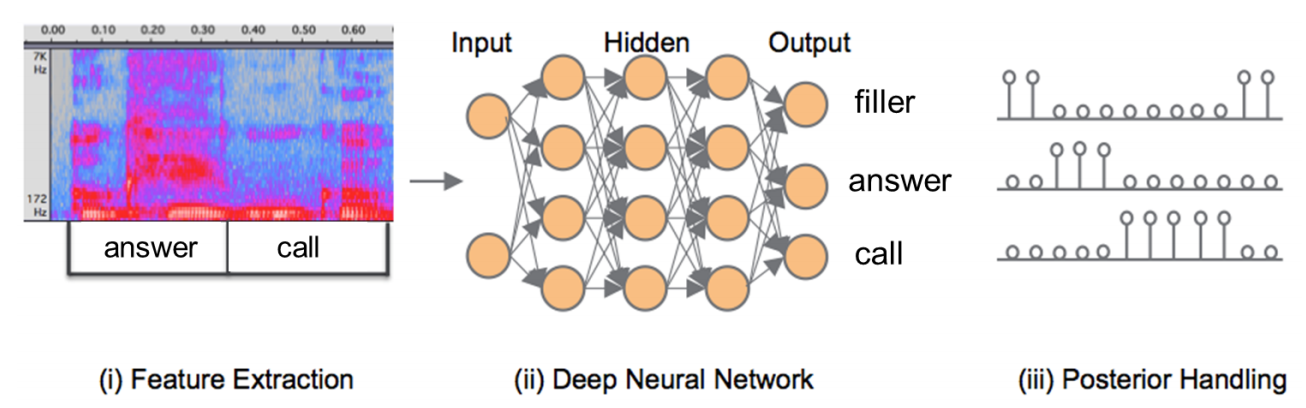
\includegraphics[width=0.75\textwidth]{img/papers/cnns_for_keyword_spotting/deep_kws_system_framework.png}
    \caption{Framework of Deep KWS system, components from
left to right: (i) Feature Extraction (ii) Deep Neural Network
(iii) Posterior Handling}
    \label{fig:deep_kws_system_frameworkl}
\end{figure}

This framework originally comes from \cite{chen2014small}. The only difference is the exchange of the DNN for a CNN.



\begin{itemize}
	\item Convolutional neural networks for small-footprint keyword spotting \cite{sainath2015convolutional}
\end{itemize}	

\textcolor{red}{Include summary about the different CNNs approaches which have been put into the 3 module framework of the below framework where the DNN has been exchanged for a CNN. How do the authors handle the long, one dimensional vector?}

\subsubsection{Small-footprint keyword spotting using deep neural networks}

\begin{itemize}
	\item Small-footprint keyword spotting using deep neural networks \cite{chen2014small}
\end{itemize}	

\textcolor{red}{Include summary about the comparison between DNNs and HMMs and the general 3 module approach here: 1. Feature extraction. 2. Deep Neural Network 3. Posterior Handling. DNNs do not need a decoding algorithm like HMMs with Viterbi which makes it low latency.}

\subsubsection{Speech Commands: A Dataset for Limited-Vocabulary Speech Recognition}


\begin{itemize}
	\item Speech Commands: A Dataset for Limited-Vocabulary Speech Recognition \cite{warden2018speech}
\end{itemize}	

\textcolor{red}{Include summary and say why the Speech Commands Dataset is a good fit for this thesis. You probably do not need a Voice-activity detection (VAD) system here.}


\textbf{Properties}

\begin{quote}
The final dataset consisted of 105,829 utterances of 35 words[...].\\
Each utterance is stored as a one-second (or less) WAVE format file, with the sample data encoded as linear 16-bit single-channel PCM values, at a 16 KHz rate. There are 2,618 speaker recorded, each with a unique eight-digit hexadecimal identifier assigned as described above. The uncompressed files take up approximately 3.8 GB on disk, and can be stored as a 2.7 GB gzip-compressed tar archive.
\end{quote}

\textbf{Top-One Error}

\begin{quote}
The standard chosen for the TensorFlow speech commands example code is to look for the ten words "Yes", "No", "Up", "Down", "Left", "Right", "On", "Off", "Stop", and "Go", and have one additional special label for "Unknown Word", and another for "Silence" (no speech detected). The testing is then done by providing equal numbers of examples for each of the twelve categories, which means each class accounts for approximately 8.3\% of the total. The "Unknown Word" category contains words randomly samples from classes that are part of the target set. The "Silence" category has one-second clips extracted randomly from the background noise audio files.
\end{quote}

\textbf{Applications}

\begin{quote}
The TensorFlow tutorial gives a variety of baseline models, but one of the goals of the dataset is to enable the creation and comparison of a wide range of models on a lot of different platforms, and version one of has enabled some interesting applications. CMSISNN [21] covers a new optimized implementation of neural network operations for ARM microcontrollers, and uses Soeech Commands to train and evaluate the results. Listening to the World [22] demonstrates how combining the dataset and UrbanSounds [23] can improve the noise tolerance of recognition models. Did you Hear That [24] uses the dataset to test adversarial attacks on voice interfaces. Deep Residual Learning for Small Footprint Keyword Spotting \cite{tang2018deep} shows how approaches learned from ResNet can produce more efficient and accurate models. Raw Waveformbased Audio Classification \cite{lee2017raw} investigates alternatives to traditional feature extraction for speech and music models. Keyword Spotting through Image Recognition \cite{gouda2018speech} looks at the effect of virtual adversarial training on the keyword task.
\end{quote}

\textbf{Evaluation}

\begin{quote}
One of this dataset's primary goals is to enable meaningful comparisons between different models' results, so it's important to suggest some precise testing protocols. As a starting point, it's useful to specify exactly which utterances can be used for training, and which must be reserved for testing, to avoid overfitting. The dataset download includes a text file called \texttt{validation\_list.txt}, which contains a list of files that are expected to be used for validating results during training, and so can be used frequently to help adjust hyperparameters and make other model changes. The \texttt{testing\_list.txt} file contains the names of audio clips that should only be used for measuring the results of trained models, not for training or validation. The set that a file belongs to is chosen using a hash function on its name. This is to ensure that files remain in the same set across releases, even as the total number in the same set across releases, even as the total number changes, so avoid set corss-contaimination when trying old models on the more recent test data. The Python implementation of the set assignment algorithm is given in the TensorFlow tutorial code [12] that is a companion to the dataset.
\end{quote}

\textbf{Historical Evaluations}

\begin{quote}
Version 1 of the dataset \cite{scd_v1} was released August 3rd 2017, and contained 64,727 utterances from 1,881 speakers. Training the default convolution model from the TensorFlow tutorial (based on Convolutional Neural Networks for Small-footprint Keyword Spotting \cite{sainath2015convolutional}) using the V1 training data gave a Top-One score of 85.4\%, when evaluated against the test set from V1. Training the same model against version 2 of the data set \cite{scd_v2}, documented in this paper, produces a model that scores 88.2\% Top-One on the training set extracted from the V2 data. A model trained on V2 data, but evaluated against the V1 test set gives 89.7\% Top-One, which indicates that the V2 training data is responsible for a substantial improvement in accuracy over V1. The full set of results are shown in Table \ref{tab:v1_v2_results}
\end{quote}


\begin{table}[]
\center
\begin{tabular}{|c|c|c|}
\hline
Data & V1 Training & V2 Training \\ \hline
V1 Test & 85.4\% & 89.7\% \\ \hline
V2 Test & 82.7\% & 88.2\% \\ \hline
\end{tabular}
\caption{Top-One accuracy evaluations using different training data}
\label{tab:v1_v2_results}
\end{table}




\begin{itemize}
	\item Convolutional recurrent neural networks for small-footprint keyword spotting \cite{arik2017convolutional}
	\item Honk: A PyTorch reimplementation of convolutional neural networks for keyword spotting \cite{tang2017honk}
	\item An experimental analysis of the power consumption of convolutional neural networks for keyword spotting \cite{tang2018experimental}
	\item Transfer learning for speech recognition on a budget \cite{kunze2017transfer}
	\item Learning and transferring mid-level image representations using convolutional neural networks \cite{oquab2014learning}
	\item Deep residual learning for small-footprint keyword spotting \cite{tang2018deep}
\end{itemize}




\section{Method}

\begin{enumerate}
	\item methodology, types of analyses, selection of the method
\end{enumerate}

\section{Set-up}

\begin{enumerate}
	\item selection of the speech data, description of the data, tuning/adaptation model parameters
	\item types of experiments (generalizations to which unseen conditions, etc. )
\end{enumerate}


\section{Experiments}



\section{Analysis and Results}


\section{Discussion}

\section{Conclusion}



\section{References}




\section{Appendix}

\begin{figure}[h]
    \centering
    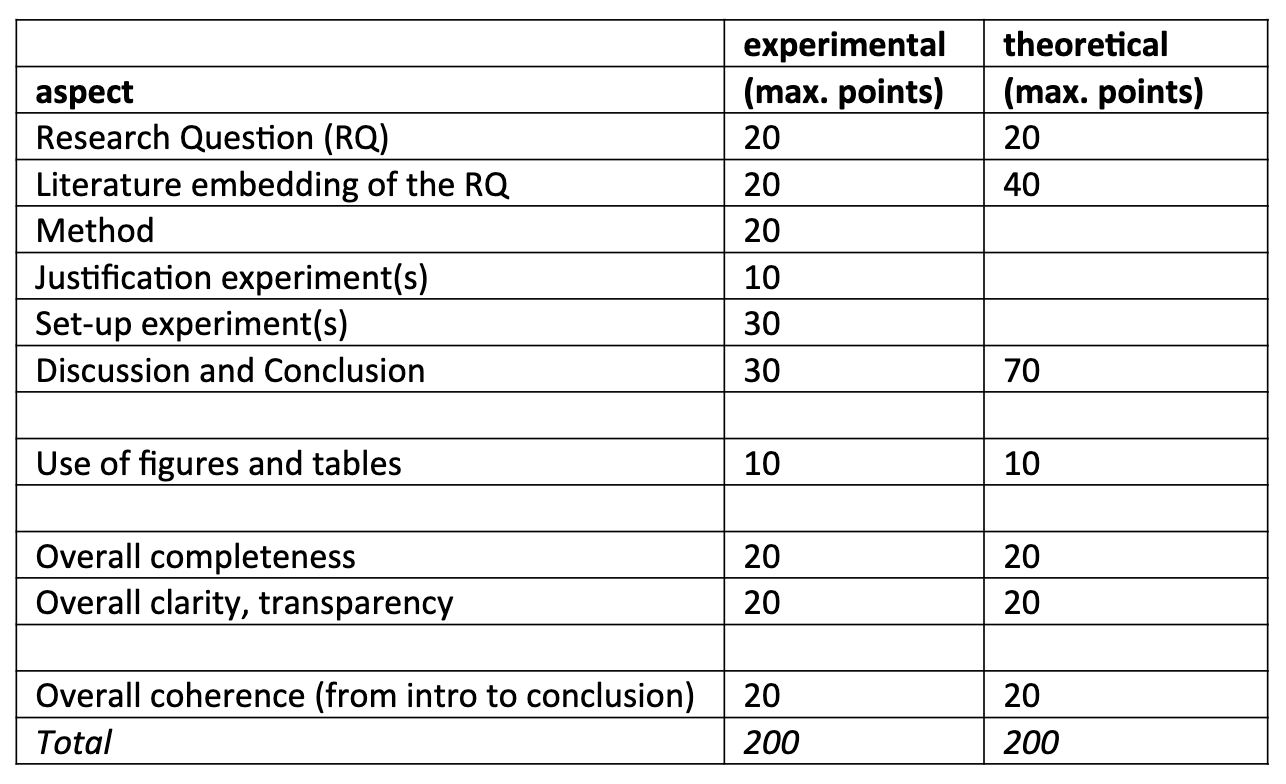
\includegraphics[width=1\textwidth]{img/grading.png}
    \caption{Weighted grading}
    \label{fig:my_label}
\end{figure}

\begin{itemize}
	\item the experiment(s) may be carried out in collaboration with others. In that case: specify in the “author’s statement” everybody’s contribution
	\item the thesis itself is written individually and assessed individually
	\item the ASR performance itself is not relevant for the assessment of the thesis
	\item the RQ, the literature embedding of the RQ, the description of the method, the justification and set-up of the experiment are relevant for the assessment 
	\item the general university guidelines apply (e.g., with respect to plagiarism)
	\item there is no minimum number of pages for the thesis
\end{itemize}



\section{Complex stuff}
\subsection{Domains}
Let's start with the following definition:
\begin{definition}\label{def:domain}
A set $U \subseteq \mathbb{C}$ is a \emph{domain} if:
\begin{itemize}
    \item $U$ is open in $\mathbb{C}$, and
    \item $U$ is connected.
\end{itemize}
\end{definition}


\subsection{Yumyumyumyum}
\towrite{an introduction and some examples}

\begin{theorem}[]
Suppose $n \in \mathbb{Z}$, then the following are equivalent:
\begin{enumerate}[label=\roman*.]
    \item $n > 5$.
    \item $5 > 5$.\todo{This doesn't seem right...}
    \item For each $n \in n$, we have:
    \begin{align}\label{eq:truth}
        n > n+1 > n+1^2 > \dots > n+7.
    \end{align}
    where $7$ is an arbitrary element of
    \begin{align*}
        \oint_{a}^{b} \supersine \alpha + i \supercosine \beta  db(a).
    \end{align*}
\end{enumerate}
\end{theorem}

\begin{remark}
Interesting!
\end{remark}
\begin{proof}
See \cite{Rynne2008LinearAnalysis}.
\end{proof}

\begin{figure}[h]
    \centering
    
\includegraphics[width=.3\textwidth]{img/in_dei_nomine_feliciter.eps}
    \caption{Motivational illustration. Similar to \cite{Oort1958,Reed1960}.}
    \label{fig:logo}
\end{figure}

\begin{corollary}
Suppose $U \subseteq \mathbb{C}$ is a domain (see Definition \ref{def:domain}), and $f: \overline{U} \rightarrow \mathbb{C}$ is continuous on $\overline{U}$ and holomorphic on $U$. If $z \mapsto |f(z)|$ is constant on $\partial U$, then $f$ has a zero in $U$.
\end{corollary}
\begin{proof}
If not, consider $\frac{1}{f}$.
\end{proof}
The proof of this theorem is illustrated in Figure \ref{fig:logo}.



\newpage

% You can choose a citation style, 'plain' is the default
% See:
% https://www.overleaf.com/learn/latex/Bibtex_bibliography_styles

\bibliographystyle{plain}
\bibliography{references.bib}

\end{document}

% Have fun!
% -fons

% http://www2.washjeff.edu/users/rhigginbottom/latex/resources/symbols.pdf